\chapter{Σχεδιασμός και αρχιτεκτονική του συστήματος}
\InitialCharacter{Σ}το κεφάλαιο αυτό περιγράφεται η αρχιτεκτονική της \en{dApp} και τα σενάρια εκτέλεσης που καλύπτει. Αρχικά, παρουσιάζεται μια επισκόπηση της λειτουργίας της εφαρμογής και των συμμετεχόντων σε αυτήν. Στην συνέχεια, αναλύονται η αρχιτεκτονική της εφαρμογής τα σενάρια εκτέλεσης που καλύπτει και οι διαδικασίες που ακολουθούνται σε κάθε ένα από αυτά. Τέλος, παρουσιάζονται τα μέτρα ασφαλείας που έχουν ληφθεί για την την διασφάλιση της αξιοπιστίας της.

\section{Επισκόπηση της προτεινόμενης \en{dApp}}

Στο πλαίσιο του αποκεντρωμένου υπολογιστικού νέφους, αναδύονται 
δύο κρίσιμες προκλήσεις: η διασφάλιση της ειλικρινούς εκτέλεσης των εργασιών 
και η προστασία του περιβάλλοντος του παρόχου. Οι παραδοσιακές μέθοδοι συχνά 
περιλαμβάνουν δυσκίνητες ή δαπανηρές διαδικασίες επαλήθευσης, οι οποίες μπορεί 
να αποτελέσουν αποτρεπτικό παράγοντα για πολλούς χρήστες. Επιπλέον η εκτέλεση 
άγνωστου κώδικα στο μηχάνημα ενός παρόχου ενέχει σημαντικούς κινδύνους ασφαλείας.

Αντιμετωπίζοντας αυτές τις προκλήσεις, η \en{dApp} εισάγει δύο απλές λύσεις:
\begin{itemize}
\item Μηχανισμός επαλήθευσης: Αντί να βασίζεται σε βαριές και δαπανηρές 
υπολογιστικές αποδείξεις, η \en{dApp} χρησιμοποιεί μια προκαθορισμένη \en{Java} κλάση. 
Οι πελάτες παρέχουν τον κώδικά τους ως μεταγλωττισμένη \en{Java} κλάση, διασφαλίζοντας 
με τον τρόπο αυτό ότι οι πάροχοι δεν μπορούν να έχουν άμεση πρόσβαση στον κώδικα 
ή να τροποποιήσουν την λογική της υλοποίησής του. Η κλάση αυτή, με την ονομασία 
\textit{\en{Code}}, πρέπει να περιέχει δύο βασικές \en{public} μεθόδους: την \textit{\en{getComputation}}, η οποία περιέχει την λογική της εκτέλεσης της υπολογιστικής εργασίας και την \textit{\en{getVerification}}, η οποία επιστρέφει μια συμβολοσειρά που έχει οριστεί από τον πελάτη. Αυτή η συμβολοσειρά επαλήθευσης λειτουργεί ως απόδειξη της πραγματικής εκτέλεσης της εργασίας, διασφαλίζοντας ότι οι πάροχοι έχουν όντως εκτελέσει τους υπολογισμούς του πελάτη.
\item Εκτέλεση εργασίας σε \en{Docker Container}: Για να διασφαλιστεί η ασφάλεια του μηχανήματος του παρόχου και να διατηρηθεί η ακεραιότητα της διαδικασίας εκτέλεσης, οι εργασίες εκτελούνται εντός ενός \en{docker container}. Αυτό το \en{containerized} περιβάλλον απομονώνει την εκτέλεση από το πρωτεύον σύστημα του παρόχου, αποτρέποντας την πρόκληση βλάβης από πιθανό κακόβουλο κώδικα. Επιπλέον, εξασφαλίζει ένα συνεπές περιβάλλον εκτέλεσης και αποτρέπει κάθε εξωτερική παρέμβαση, διασφαλίζοντας ότι η εργασία εκτελείται όπως προβλέπεται από τον πελάτη 
\end{itemize}

Με αυτές τις απλές και οικονομικά αποδοτικές λύσεις, η \en{dApp} στοχεύει στον εκδημοκρατισμό και την ενίσχυση της προσβασιμότητας του υπολογιστικού νέφους, δρώντας ως γέφυρα μεταξύ των πελατών που έχουν υπολογιστικές εργασίες και των παρόχων που κατέχουν τους πόρους για την εκτέλεσή τους. Εξασφαλίζοντας την διαφανή και επαληθεύσιμη εκτέλεση των εργασιών, η \en{dApp} προσφέρει και αξιοπιστία στις διαδικασίες εκτέλεσης και πληρωμής.

Για να κατανοηθεί καλύτερα ο τρόπος λειτουργίας του αποκεντρωμένου συστήματος, παρακάτω προσδιορίζονται οι κύριοι συμμετέχοντες σε αυτό.

\section{Περιγραφή των συμμετεχόντων}
Οι οντότητες που συμμετέχουν στην εφαρμογή είναι οι ακόλουθες:
\begin{itemize}
    \item Πελάτης (\en{client}): Οντότητα που απαιτεί την εκτέλεση υπολογιστικών εργασιών. 
    Παρέχει την εργασία με την μορφή μεταγλωττισμένης κλάσης \en{Java} και ξεκινά την διαδικασία δημοπρασίας για την εύρεση κατάλληλου παρόχου. Στην συνέχεια επιλέγει τον πάροχο που επιθυμεί από αυτούς που έχουν υποβάλλει προσφορά και, όταν η εκτέλεση της εργασίας του ολοκληρωθεί, πραγματοποιεί την πληρωμή και λαμβάνει τα αποτελέσματα των υπολογισμών του.
    \item Πάροχος (\en{provider}): Οντότητα με υπολογιστικούς πόρους που επιθυμεί να εκτελέσει εργασίες για τους πελάτες. Υποβάλλουν προσφορές για εργασίες σε δημοπρασία και, αφού επιλεγούν, εκτελούν τις εργασίες σε ασφαλές περιβάλλον.
\end{itemize}    

\begin{illustration}
    \centering
    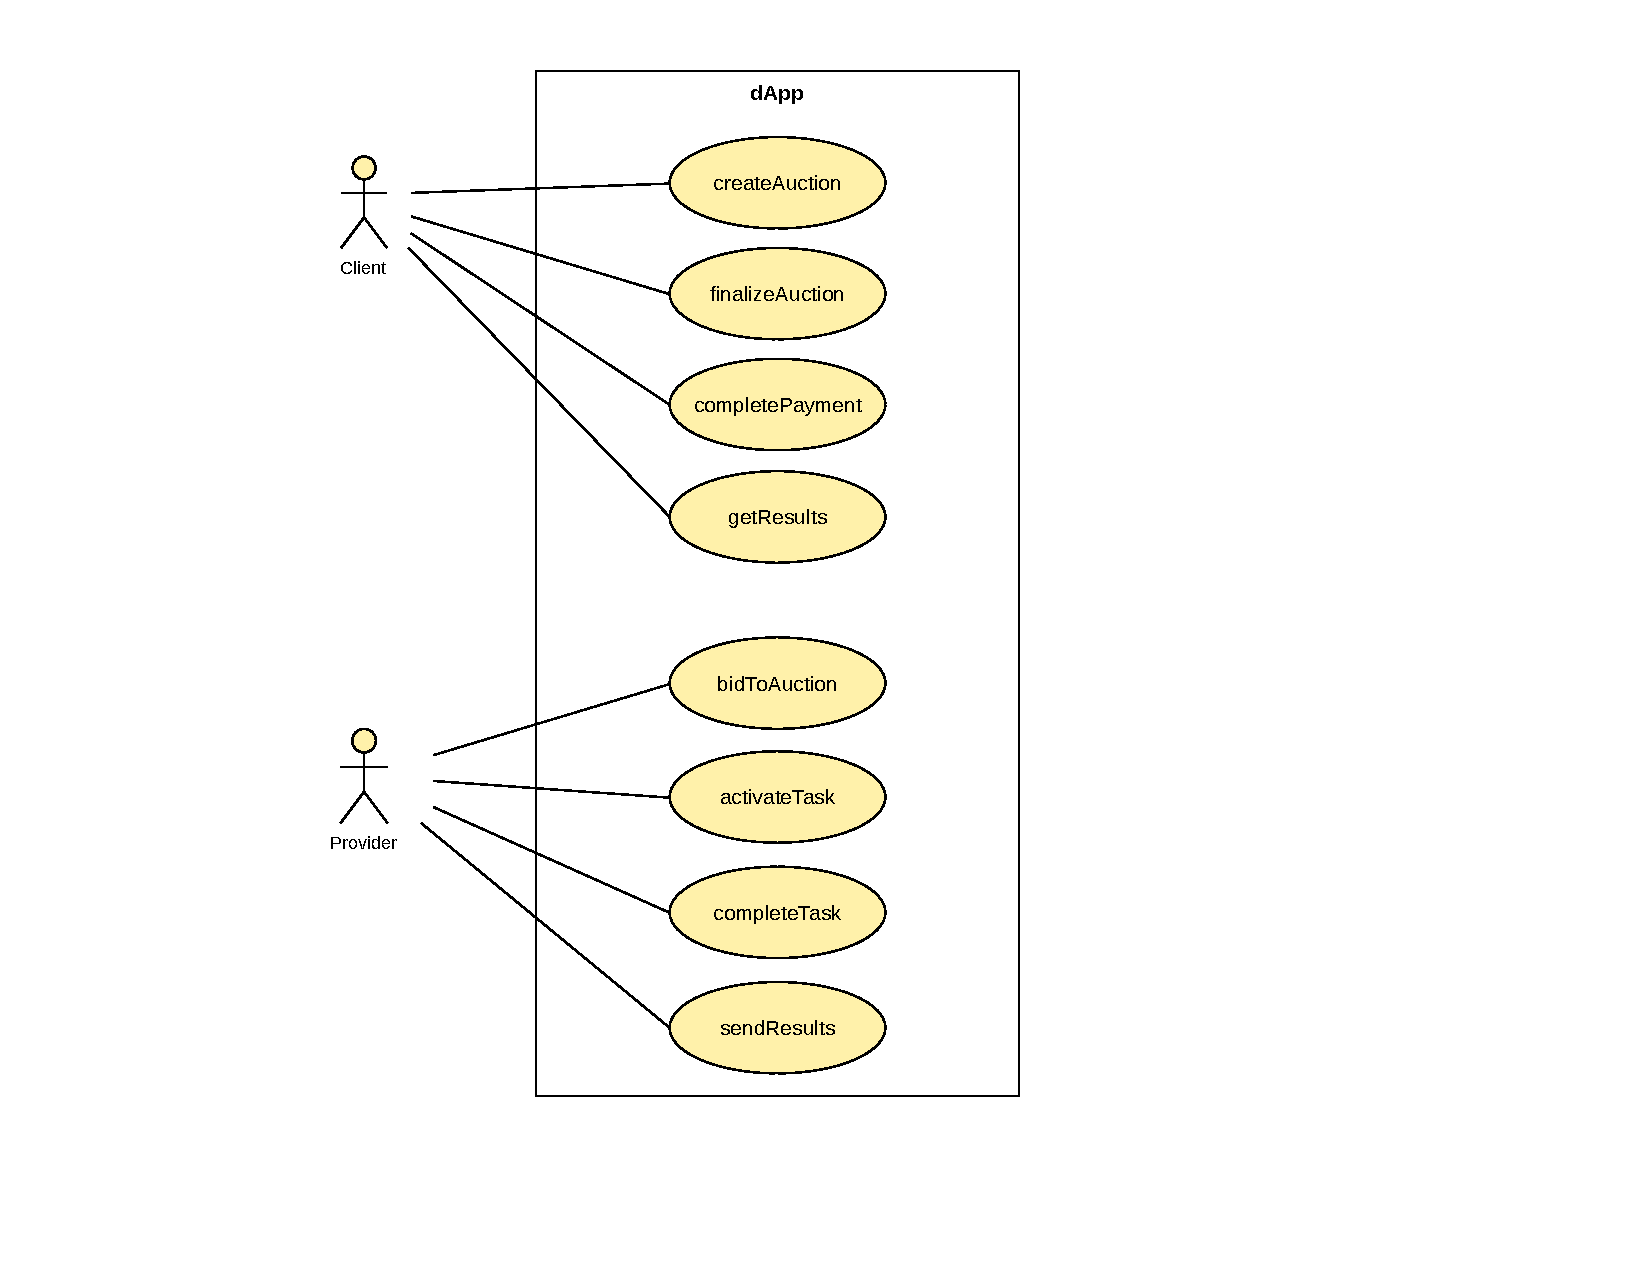
\includegraphics[width=0.5\textwidth]{figures/figure-003.pdf}
    \caption{\en{Use case diagram} της \en{dApp}} 
\end{illustration}

Με σαφή κατανόηση των ρόλων των πελατών και των παρόχων, παρακάτω αναλύεται η τεχνική αρχιτεκτονική που διευκολύνει τις αλληλεπιδράσεις τους και διασφαλίζει την σταθερότητα του συστήματος.

\section{Αρχιτεκτονική του συστήματος}
Η αρχιτεκτονική της \en{dApp} έχει σχεδιαστεί για να διευκολύνει την απρόσκοπτη αλληλεπίδραση μεταξύ πελατών και παρόχων, διασφαλίζοντας παράλληλα την ακεραιότητα και την ασφάλεια των υπολογιστικών εργασιών. 
Ακολουθεί μια ανάλυσή της:
\begin{enumerate}
    \item \en{Smart Contracts}:
        \begin{itemize}
            \item[-] \en{AuctionsManager}: Έξυπνο συμβόλαιο, το οποίο διαχειρίζεται τη διαδικασία δημοπρασίας, από την έναρξή της από τον πελάτη έως την επιλογή ενός παρόχου με βάση τις προσφορές. Χειρίζεται τις προθεσμίες και άλλες παραμέτρους που αφορούν τη δημοπρασία.
            \item[-] \en{TasksManager}: Έξυπνο συμβόλαιο, το οποίο επιβλέπει τον κύκλο ζωής μιας υπολογιστικής εργασίας. Εξασφαλίζει τις διαδικασίες σωστής εκτέλεσης, επαλήθευσης και πληρωμής και διαχειρίζεται επίσης τις χρηματικές εγγυήσεις και τις προθεσμίες που σχετίζονται με κάθε εργασία.
        \end{itemize}
    \item Ενσωμάτωση \en{IPFS}:
        \begin{itemize}
            \item[-] Οι πελάτες μεταφορτώνουν τη μεταγλωττισμένη κλάση \en{Java} (\en{Code.class}) στο \en{IPFS (InterPlanetary FileSystem )} και παρέχουν το \en{CID (Content Identifier)} κατά τη δημιουργία της δημοπρασίας. Αυτό διασφαλίζει ότι ο κώδικας παραμένει αμετάβλητος και προσβάσιμος στον επιλεγμένο πάροχο. 
            \item[-] Οι τυποποιημένες \en{boilerplate} κλάσεις (\en{Main.class} και \en{Time.class}) αποθηκεύονται επίσης στο \en{IPFS} και ανακτώνται χρησιμοποιώντας προκαθορισμένα \en{CID}. 
        \end{itemize}
    \item \en{Docker Container}: 
    \begin{itemize} 
        \item[-] Το \en{Docker  container} χρησιμεύει ως περιβάλλον εκτέλεσης των υπολογιστικών εργασιών. Αποτελείται από δύο πρωταρχικά \en{images}:
        \begin{itemize}
            \item[-] \en{Java Image}: Εκτελεί την \en{Main.class}, η οποία ενορχηστρώνει ολόκληρη τη διαδικασία, από την εκτέλεση της υπολογιστικής εργασίας του πελάτη έως τον υπολογισμό διάρκειάς της και τέλος την εκτύπωση των αποτελεσμάτων.
            \item[-] \en{Node Image}: Μια ειδική ελαφριά έκδοση της \en{dApp} εκτελείται μέσα σε αυτό το \en{docker image}. Αναλύει τα αποτελέσματα από την εκτέλεση της \en{Java class} και τα στέλνει στο έξυπνο συμβόλαιο \en{TasksManager}. Επίσης αποθηκεύει το αποτέλεσμα της εκτέλεσης της εργασίας σε ένα αρχείο στο μηχάνημα του παρόχου ώστε στην συνέχεια να σταλεί στο \en{IPFS} από την \en{dApp}.
        \end{itemize}
    \end{itemize}
    \item Γραφική διεπαφή:
        \begin{itemize}
            \item[-] Κατασκευασμένη με τη χρήση του \en{React Framework}, η διεπαφή της \en{dApp} διευκολύνει τις αλληλεπιδράσεις του χρήστη με το σύστημα. Επιτρέπει στους πελάτες να ξεκινούν δημοπρασίες, στους παρόχους να υποβάλλουν προσφορές και στα δύο μέρη να διαχειρίζονται και να παρακολουθούν τις εργασίες που συμμετέχουν. Η διεπαφή χειρίζεται επίσης τον κατακερματισμό της συμβολοσειράς επαλήθευσης και αλληλεπιδρά με το \en{Ethereum blockchain} μέσω \en{events} που στέλνονται από τα \en{smart contracts}. 
        \end{itemize}
    \item Μηχανισμός επαλήθευσης:
     \begin{itemize}
        \item[-] Όπως αναλύθηκε προηγουμένως, ο μηχανισμός επαλήθευσης διασφαλίζει ότι οι πάροχοι εκτελούν πραγματικά την υπολογιστική εργασία του πελάτη. Η μέθοδος \en{getVerification} στην \en{Code.class} επιστρέφει μια συμβολοσειρά που ορίζεται από τον πελάτη, η οποία, όταν κατακερματιστεί και συγκριθεί με τον αποθηκευμένο κατακερματισμό που δηλώθηκε από τον πελάτη στο συμβόλαιο \en{AuctionsManager}, επαληθεύει την ορθή εκτέλεση της εργασίας.
     \end{itemize}
    \item Σύστημα πληρωμών και εγγυήσεων: 
    \begin{itemize}
        \item[-] Τόσο οι πελάτες όσο και οι πάροχοι τοποθετούν χρηματικές εγγυήσεις για να διασφαλίσουν τη δέσμευσή τους στην εργασία. Μετά την επιτυχή ολοκλήρωση και επαλήθευση της εργασίας, ο πελάτης πληρώνει τον πάροχο με βάση το συμφωνημένο ποσο (\en{Gwei} ανά δευτερόλεπτο εκτέλεσης) και την διάρκεια της εκτέλεσης. Τα προαναφερθέντα έξυπνα συμβόλαια χειρίζονται αυτές τις συναλλαγές, εξασφαλίζοντας διαφάνεια και ασφάλεια.
    \end{itemize}
\end{enumerate}

\begin{illustration}
    \centering
    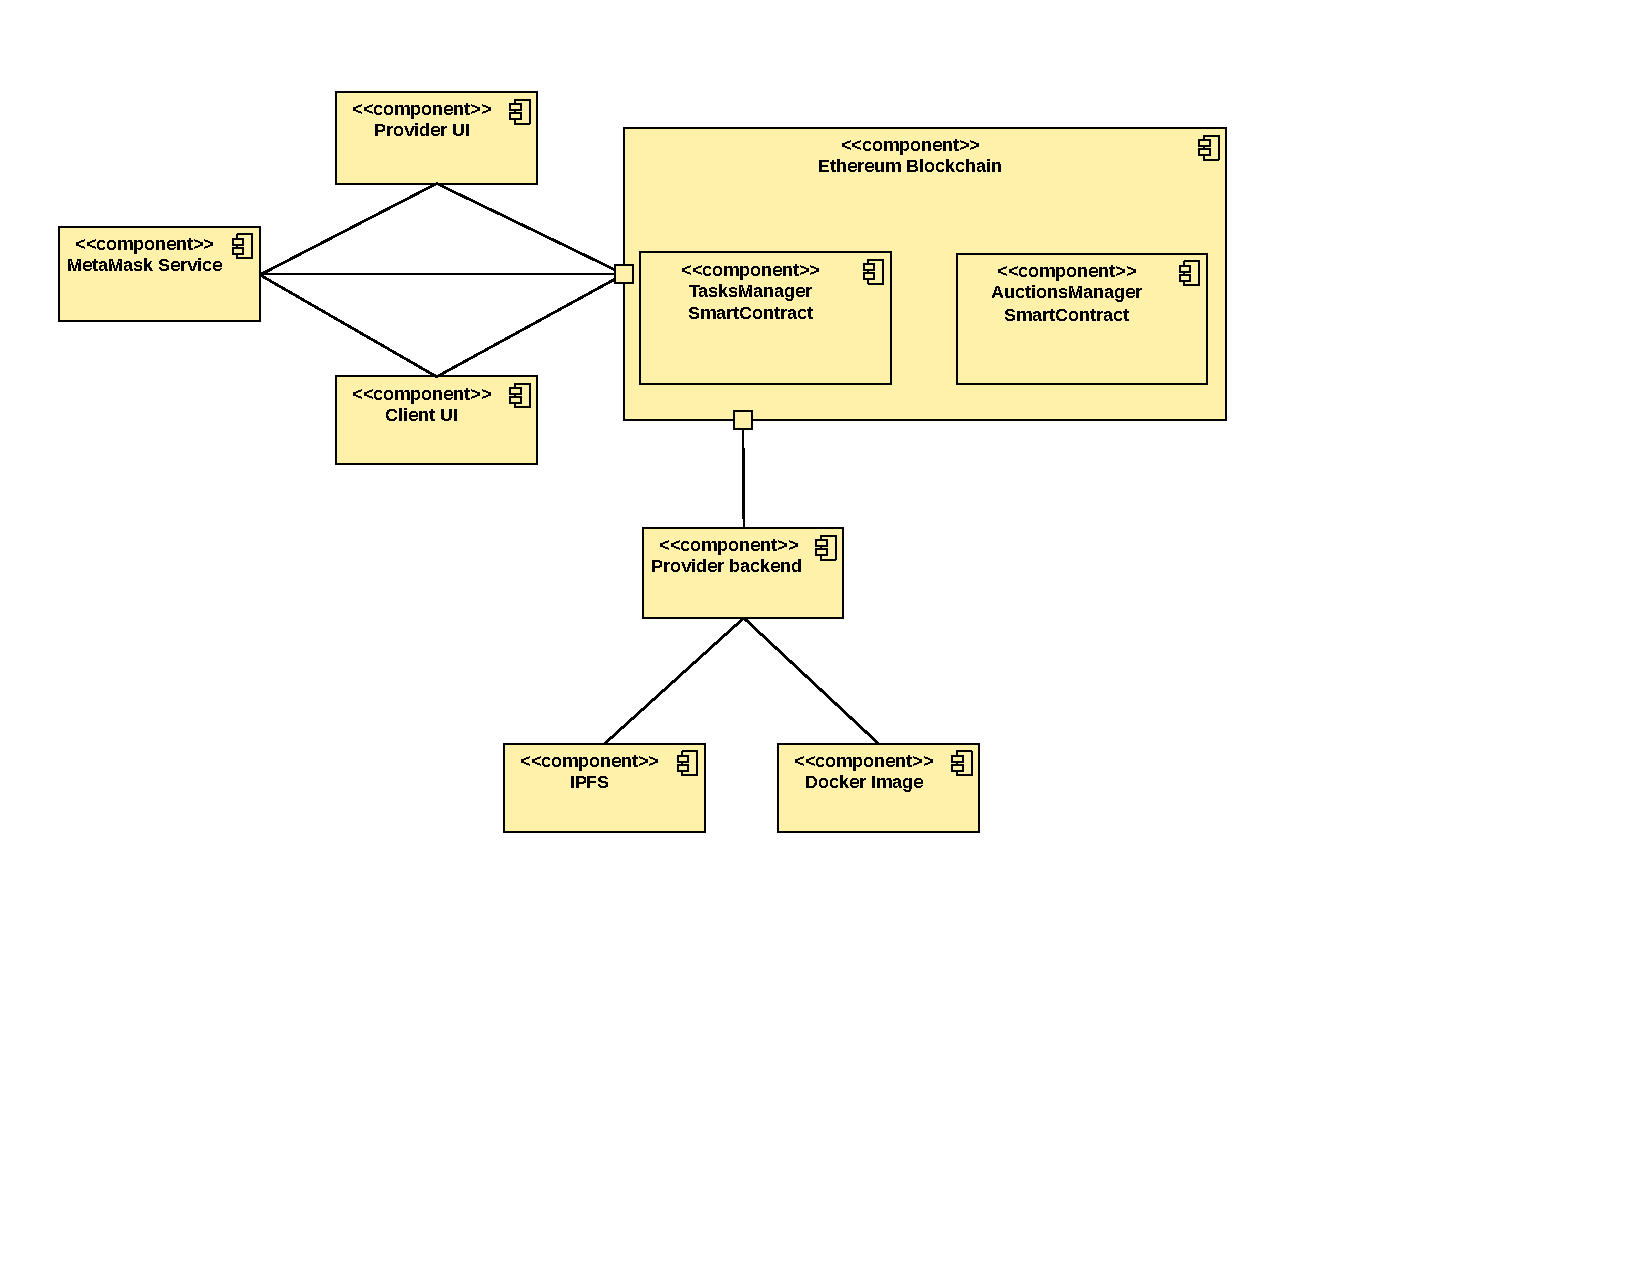
\includegraphics[width=0.8\textwidth]{figures/figure-004.pdf}
    \caption{\en{Component diagram} της \en{dApp}} 
\end{illustration}

Με την ενσωμάτωση αυτών των στοιχείων, η αρχιτεκτονική της \en{dApp} εξασφαλίζει ένα στιβαρό, ασφαλές και αποτελεσματικό σύστημα για αποκεντρωμένο υπολογιστικό νέφος. 

Ο σχεδιασμός δίνει προτεραιότητα στην αξιοπιστία, διασφαλίζοντας ότι τόσο οι πελάτες όσο και οι πάροχοι μπορούν να συμμετέχουν σε υπολογιστικές εργασίες με εμπιστοσύνη.

Η αρχιτεκτονική παρέχει ένα σχέδιο του συστήματος, δίνοντας έμφαση στα συστατικά του 
και στις αλληλεπιδράσεις τους. 

Παρακάτω παρουσιάζεται η συμπεριφορά του συστήματος τόσο στο πρωταρχικό σενάριο εκτέλεσής του, όσο και στα εναλλακτικά μη ιδανικά σενάρια.

\section{Ροές εργασιών του συστήματος}
\subsection{Επιτυχής ολοκλήρωση εργασίας }
Τα βήματα που ακολουθούνται έως την επιτυχή ολοκλήρωση μιας εργασίας είναι τα ακόλουθα:
\begin{enumerate}
    \item Δημιουργία εργασιών: Ο πελάτης γράφει και μεταγλωττίζει την κλάση \en{Java} με το όνομα \textit{\en{Code}}. Η κλάση αυτή περιέχει δύο \en{public} μεθόδους: την \textit{\en{getComputation}} που περιέχει τη λογική της εργασίας και την \textit{\en{getVerification}} που επιστρέφει μια προκαθορισμένη συμβολοσειρά για επαλήθευση. Η κλάση \textit{\en{getComputation}} έχει επιλεγεί να επιστρέφει \en{String} για συμβατότητα της \en{Main.class} με κάθε συνάρτηση υπολογισμού.
    \item \en{IPFS Upload}: Ο πελάτης μεταφορτώνει την μεταγλωττισμένη κλάση του στο \en{IPFS} (\en{InterPlanetary FileSystem}) και λαμβάνει ένα \en{CID} (\en{Content Identifier}).
    \item Έναρξη δημοπρασίας: Χρησιμοποιώντας την \en{dApp}, ο πελάτης ξεκινά μια δημοπρασία, παρέχοντας τις απαραίτητες λεπτομέρειες, όπως η προθεσμία της δημοπρασίας, η προθεσμία εκτέλεσης της εργασίας, το \en{CID} της \en{Java} κλάσης και την συμβολοσειρά επαλήθευσης.
    \item Υποβολή προσφοράς: Οι πάροχοι υποβάλλουν προσφορά για την εργασία καθορίζοντας την τιμή (σε \en{Gwei} ανά δευτερόλεπτο εκτέλεσης) που προτείνουν.
    \item Επιλογή παρόχου: Ο πελάτης επιλέγει τον πάροχο που επιθυμεί να εκτελέσει την εργασία του, βασιζόμενος στην τιμή προσφοράς και στην βαθμολογία που έχει προκύψει από προηγούμενες επιδόσεις του παρόχου. Στο βήμα αυτό, ο πελάτης στέλνει ως εγγύηση το ποσό που αντιστοιχεί σε 2 δευτερόλεπτα εκτέλεσης της εργασίας.
    \item Ενεργοποίηση της εργασίας: Ο πάροχος ενεργοποιεί την εργασία στέλνοντας την δική του εγγύηση, η οποία αντιστοιχεί σε 10 δευτερόλεπτα εκτέλεσης της εργασίας. Στην συνέχεια, το \en{dApp} ενορχηστρώνει την διαδικασία εκτέλεσης της εργασίας, λαμβάνοντας από το \en{IPFS} τις απαραίτητες κλάσεις, δημιουργώντας την εικόνα \textit{\en{Docker}} και εκκινώντας τον \en{docker container}.
    \item Εκτέλεση εργασίας: Εντός του \en{docker container}, εκτελείται η κλάση \en{Java}. Η συμβολοσειρά επαλήθευσης, μαζί με την διάρκεια εκτέλεσης και τον χρόνο ολοκλήρωσης της εργασίας στέλνονται στο \en{smart contract} \textit{\en{TasksManager}} για τον έλεγχο της διαδικασίας. Τα αποτελέσματα του υπολογισμού εγγράφονται σε ένα αρχείου κειμένου. Το συμβόλαιο επαληθεύει την ορθή εκτέλεση της εργασίας με βάση την παρεχόμενη συμβολοσειρά επαλήθευσης και διασφαλίζει ότι ολοκληρώθηκε εντός της συμφωνημένης προθεσμίας. Στην περίπτωση ορθής και έγκαιρης εκτέλεσης, η βαθμολογία του παρόχου αυξάνεται και οι χρηματικές εγγυήσεις του επιστρέφονται.
    \item Υποβολή αποτελέσματος: To \en{dApp} μεταφορτώνει εκ μέρους του παρόχου το αποτέλεσμα της εργασίας στο \en{IPFS} και υποβάλλει το \en{CID} στο \en{smart contract} \textit{\en{TasksManager}}.
    \item Πληρωμή: Μετά την επιτυχή εκτέλεση και υποβολή των αποτελεσμάτων από τον πάροχο, ο πελάτης ενημερώνεται για το ποσό που οφείλει να πληρώσει, με βάση την διάρκεια εκτέλεσης της εργασίας. Στην συνέχεια αποστέλλει στο \en{smart contract} \textit{\en{TasksManager}} το ποσό της πληρωμής που εκκρεμεί και τότε μπορεί να αποκτήσει πρόσβαση στο \en{CID} των αποτελεσμάτων. Με την επιτυχημένη ολοκλήρωση της πληρωμής η βαθμολογία του πελάτη αυξάνεται, ως δείκτης φερεγγυότητας.
    \item Λήψη αποτελεσμάτων: Μετά την ολοκλήρωση της πληρωμής, ο πελάτης λαμβάνει το \en{CID} των αποτελεσμάτων της εκτέλεσης της υπολογιστικής του εργασίας και μπορεί να τα ανακτήσει από το \en{IPFS}.
\end{enumerate}

\subsection{Εναλλακτικές ροές εργασιών}
\subsubsection{Ανεπιτυχής ολοκλήρωση της εργασίας λόγω ασυμφωνίας επαλήθευσης \\ή καθυστερημένης εκτέλεσης}
Κατά τη λήψη των αποτελεσμάτων από τον πάροχο, το \en{smart contract TasksManager} κατακερματίζει και ελέγχει την συμβολοσειρά επαλήθευσης.
Εάν η κατακερματισμένη συμβολοσειρά επαλήθευσης δεν ταιριάζει με αυτήν που παρέχεται από τον πελάτη, η εργασία θεωρείται ανεπιτυχής.

Ταυτόχρονα, ελέγχεται και ο χρόνος ολοκλήρωσης της εκτέλεσης. Εάν η εργασία ολοκληρώθηκε μετά τη συμφωνηθείσα προθεσμία, θεωρείται επίσης ανεπιτυχής.

Και στις δύο περιπτώσεις ανεπιτυχούς επαλήθευσης ή καθυστερημένης εκτέλεσης, η βαθμολογία του παρόχου μειώνεται, ενώ οι χρηματικές εγγυήσεις του χάνονται και παραμένουν στο έξυπνο συμβόλαιο \en{TasksManager}. Στον πελάτη επιστρέφονται οι δικές του χρηματικές εγγυήσεις.

\subsubsection{Καθυστέρηση του παρόχου στην υποβολή των αποτελεσμάτων}
Μετά την επιτυχημένη εκτέλεση της εργασίας, ο πάροχος έχει περιθώριο μίας ημέρας για να υποβάλει τα αποτελέσματα στο έξυπνο συμβόλαιο \en{TasksManager}. Εάν ο πάροχος δεν υποβάλει τα αποτελέσματα εντός αυτού του χρονικού διαστήματος, η βαθμολογείται αρνητικά και χάνει τις χρηματικές εγγυήσεις του, οι οποίες παραμένουν στο συμβόλαιο. Παράλληλα, επιστρέφονται στον πελάτη οι δικές του χρηματικές εγγυήσεις.

\subsubsection{Δικαίωμα ακύρωσης του πελάτη πριν από την ενεργοποίηση της \\εργασίας}
Μέχρι ο πάροχος να ενεργοποιήσει την υπολογιστική εργασία, ο πελάτης έχει το δικαίωμα να την ακυρώσει. Κατά την ακύρωση, οι εξασφαλίσεις του πελάτη επιστρέφονται. Στο βήμα αυτό ο πάροχος δεν έχει αποστείλει ακόμα τις δικές του χρηματικές εγγυήσεις ώστε να του επιστραφούν.

\subsubsection{Δικαίωμα ακύρωσης του πελάτη για καθυστερημένη ολοκλήρωση}
Στην περίπτωση που έχει παρέλθει ο χρόνος της προσυμφωνημένης προθεσμίας για την εκτέλεση της υπολογιστικής εργασίας, δίνοντας ακόμη περιθώριο μιας ημέρας, ο πελάτης έχει το δικαίωμα να ακυρώσει την εργασία. Στην περίπτωση αυτή, μεταφέρεται στον πελάτη τόσο η δική του χρηματική εγγύηση, όσο και του παρόχου. 

\subsubsection{Μη ολοκλήρωση πληρωμής από τον πελάτη}
Στην περίπτωση επιτυχημένης εκτέλεσης της εργασίας εκ μέρους του παρόχου, ο πελάτης έχει το περιθώριο μιας ημέρας για να ολοκληρώσει την πληρωμή. Αν αυτό δεν συμβεί, ο πάροχος έχει το δικαίωμα να τον καταγγείλει. Τότε η βαθμολογία του πελάτη μειώνεται, ως δείγμα αφερεγγυότητας. \\

Παρακάτω παρουσιάζεται το \en{Activity Diagram} της \en{dApp} για τις βασικές ροές εκτέλεσής της.
\begin{illustration}
    \centering
    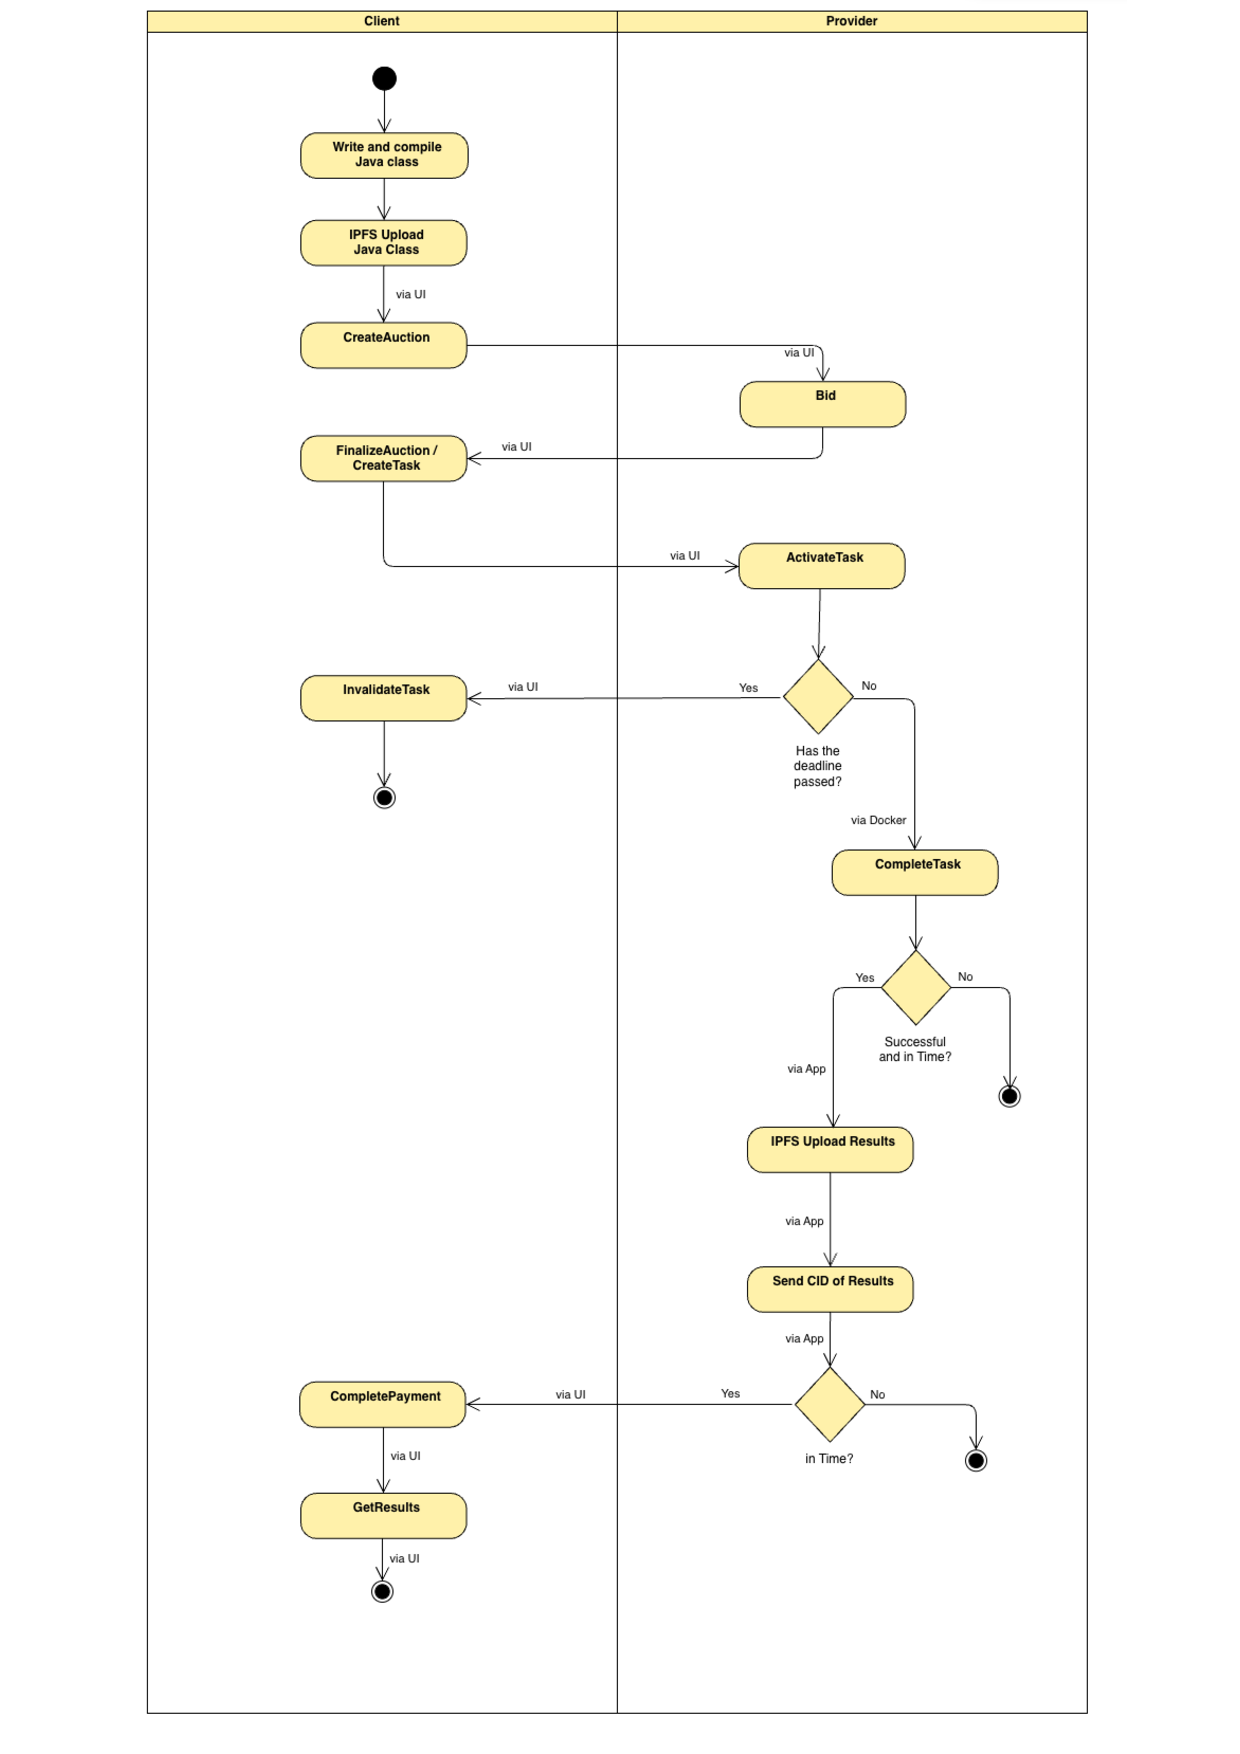
\includegraphics[width=1.1\textwidth]{figures/figure-005.pdf}
    \caption{\en{Activity diagram} της \en{dApp}} 
\end{illustration}

\newpage
Ενώ οι εναλλακτικές ροές εξασφαλίζουν ευελιξία και ευρωστία σε διάφορα σενάρια, το θεμέλιο αυτής της \en{dApp} έγκειται στα μέτρα ασφαλείας της. Τα μέτρα αυτά όχι μόνο προστατεύουν τα συμφέροντα των πελατών και των παρόχων, αλλά διασφαλίζουν επίσης τη συνολική αξιοπιστία του συστήματος. 

Παρακάτω παρουσιάζονται οι μηχανισμοί ασφάλειας της \en{dApp}.


\section{Μέτρα ασφαλείας για τη διασφάλιση της αξιοπιστίας}
Η αξιοπιστία του συστήματος διασφαλίζεται εφαρμόζοντας τα ακόλουθα μέτρα:
\begin{itemize}
\item[-] Συμβολοσειρά επαλήθευσης: Ο πελάτης παρέχει μια συμβολοσειρά επαλήθευσης που επιθυμεί, η οποία κατακερματίζεται (πραγματοποιείται \en{hash} με τον αλγόριθμο \en{keccak256} που χρησιμοποιεί το \en{Ethereum virtual machine}) και αποθηκεύεται στο έξυπνο συμβόλαιο. Αυτό διασφαλίζει ότι ο πάροχος έχει εκτελέσει πραγματικά την εργασία, καθώς για την επαλήθευση πρέπει να επιστρέψει στο συμβόλαιο την σωστή συμβολοσειρά στην αρχική της μορφή (πριν κατακερματιστεί) χωρίς να έχει άμεση πρόσβαση σε αυτή.
\item[-] \en{Docker containerization}: Για να διασφαλιστεί η ασφάλεια του μηχανήματος του παρόχου και να αποτραπεί η αλλοίωση της εκτέλεσης από αυτόν, οι εργασίες εκτελούνται σε \en{docker containers}. Η ενθυλάκωση αυτή εξασφαλίζει ένα συνεπές και απομονωμένο περιβάλλον για την εκτέλεση των εργασιών.
\item[-] \en{Blockchain}: Όλες οι αλληλεπιδράσεις, από την έναρξη της δημοπρασίας έως την ολοκλήρωση της εργασίας, καταγράφονται στο \en{Blockchain}. Αυτό διασφαλίζει τη διαφάνεια και επιτρέπει στους ενδιαφερόμενους να επαληθεύουν όλες τις ενέργειες. 
\item[-] Μηχανισμός εγγυήσεων:  Τόσο ο πελάτης όσο και ο πάροχος αποστέλλουν χρηματικές εγγυήσεις στο έξυπνο συμβόλαιο. Αυτό λειτουργεί ως δέσμευση και διασφαλίζει ότι και τα δύο μέρη ενεργούν με ειλικρίνεια και έχουν κίνητρο για την επιτυχή ολοκλήρωση της διαδικασίας, καθώς σε περίπτωση ασυμφωνίας στην οποία ευθύνονται μπορεί να χάσουν τις εγγυήσεις τους. 
\item[-] Επικοινωνία μέσω \en{events}: Η \en{dApp} και τα έξυπνα συμβόλαια επικοινωνούν μέσω \en{events} που παρέχουν τα συμβόλαια. Αυτό διασφαλίζει ότι όλα τα ενδιαφερόμενα μέρη ενημερώνονται άμεσα για τα διάφορα στάδια του κύκλου ζωής της εργασίας. 
\end{itemize}

Με την ενσωμάτωση αυτών των μέτρων ασφαλείας, η \en{dApp} διασφαλίζει ένα αξιόπιστο περιβάλλον τόσο για τους πελάτες όσο και για τους παρόχους, προωθώντας τη δίκαιη και διαφανή εκτέλεση των υπολογιστικών εργασιών.